%%%%%%%%%% Page 3 - Col 1 %%%%%%%%%%
\newpage
\colorfulheader{machine learning}

\begin{minipage}[t]{0.485\textwidth}
    \textbf{Neural Network} is an object that tries to mimic the human brain by using \textbf{various layers} that perform a particular task. Each layer consists of neurons that get activated under certain circumstances (simulating \textit{stimuli}). Neuron are \textbf{inter-connected} between layers (via \textbf{weights}) which are powered by \textbf{activation functions}.\\

    The information passing from one layer to another is called \textbf{forward propagation}. On the other hand, \textbf{back propagation} is the action of updating the weights to reduce the loss function via an optimizer (the most common one being \textbf{gradient descent}). A step to simulate input to output (across the data set) is denoted as \textbf{epoch}.\\

    An activation function task is to transform a given input to a required output introducing non-linearities (without it the network would behave like a linear regression with limited learning and unable to be used in \textbf{images}, \textbf{videos}, \textbf{audio}, etc.)\\

    For Convolutional Neural Networks (\textbf{CNN}) some relevant layers
    \begin{itemize}
        \setlength\itemsep{0pt}
        \item \textbf{Pooling}. One \textit{accumulates} features to reduce the spatial size of the network and reduce amount of parameters (e.g. max, average, general, etc.)
        \item \textbf{Convolution}. It uses a \textit{kernel} to apply over an input signal and return relevant information from it (e.g. image processing, Fourier transform, moving averages, etc.)
        \item \textbf{Dropout}. Randomly replaced some of the elements of an input by 0 with a given \textit{probability}.
    \end{itemize}
    \textbf{Mask RCNN} (Region-Based Convolutional Neuronal Network) is a state-of-the-art \textbf{deep learning} framework for instance segmentation in computer vision. It is done by adding \textit{Fully Convolutional Networks} to \textit{Faster R-CNN}
    \begin{customcenter}[3pt]
        \begin{tikzpicture}
            \tikzstyle{arrow}=[thick,->,>=stealth]
            \tikzstyle{rcnnnode1} = [minimum width=6cm,fill=ProcessBlue!40,rounded corners,text=black]
            \tikzstyle{rcnnnode2} = [minimum width=2.5cm,fill=ProcessBlue!40,rounded corners,text=black]
            \node (rcnn1) [rcnnnode1] at (0,0) {Backbone};
            \node (rcnn2) [rcnnnode2,below of=rcnn1,xshift=1cm] {$\substack{\text{RPN}\\\text{Region Proposal Network}}$ };
            \node (rcnn3) [rcnnnode1,below of=rcnn2,xshift=-1cm] {$\substack{\text{RoIAlign}\\\text{Region Of Interest Alignment}}$};
            \node (rcnn4) [rcnnnode2,below of=rcnn3,xshift=-1.55cm] {Object Detection};
            \node (rcnn5) [rcnnnode2,below of=rcnn3,xshift=+1.55cm] {Mask Generation};
            \draw [arrow] ([xshift=1cm]rcnn1.south) -- ([xshift=1cm]rcnn1.south |- rcnn2.north);
            \draw [arrow] ([xshift=-2cm]rcnn1.south) -- ([xshift=-2cm]rcnn1.south |- rcnn3.north);
            \draw [arrow] ([xshift=1cm]rcnn2.south) -- ([xshift=1cm]rcnn2.south |- rcnn3.north);
            \draw [arrow] ([xshift=1cm]rcnn3.south) -- ([xshift=1cm]rcnn3.south |- rcnn5.north);
            \draw [arrow] ([xshift=-2cm]rcnn3.south) -- ([xshift=-2cm]rcnn3.south |- rcnn4.north);
        \end{tikzpicture}
    \end{customcenter}
\end{minipage}
%%%%%%%%%%%%%%%%%%%%%%%%%%%%%%%%%%%%
\hspace{10pt}
%%%%%%%%%% Page 3 - Col 2 %%%%%%%%%%
\begin{minipage}[t]{0.485\textwidth}
    % neural network visual representation
    \begin{customcenter}[0pt]
        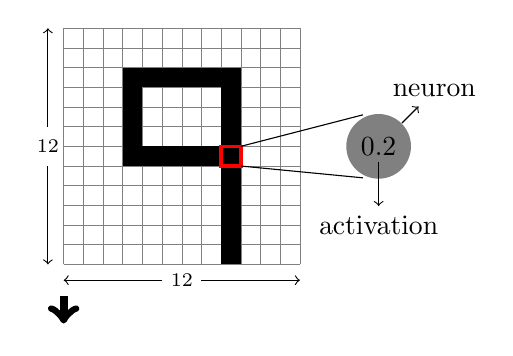
\begin{tikzpicture}
            \tikzstyle{arrow}=[thick,->,>=stealth]
            % grid of pixels
            \draw[step=0.25cm,gray,very thin] (0,0) grid (3,3);
            \draw[<-] (0.00,-0.2) -- (1.25,-0.2);
            \draw[->] (1.75,-0.2) -- (3.00,-0.2);
            \node at (1.5,-0.2) {\scriptsize 12};
            \draw[<-] (-0.2,0.00) -- (-0.2,1.25);
            \draw[->] (-0.2,1.75) -- (-0.2,3.00);
            \node at (-0.2,1.5) {\scriptsize 12};
            % neuron diagram
            \node[circle,fill=gray] (ns) at (4,1.5) {0.2};
            \node[above right of=ns] (neuron_annotation) {neuron};
            \node[below of=ns] (activation_annotation) {activation};
            \draw[->] (ns) -> (neuron_annotation);
            \draw[->] (4,1.3) -> (activation_annotation);
            % edge 1
            \fill[black] (0.75,2.25) rectangle (1.00,2.50);
            \fill[black] (1.00,2.25) rectangle (1.25,2.50);
            \fill[black] (1.25,2.25) rectangle (1.50,2.50);
            \fill[black] (1.50,2.25) rectangle (1.75,2.50);
            \fill[black] (1.75,2.25) rectangle (2.00,2.50);
            \fill[black] (2.00,2.25) rectangle (2.25,2.50);
            % edge 2
            \fill[black] (0.75,1.25) rectangle (1.00,1.50);
            \fill[black] (0.75,1.50) rectangle (1.00,1.75);
            \fill[black] (0.75,1.75) rectangle (1.00,2.00);
            \fill[black] (0.75,2.00) rectangle (1.00,2.25);
            % edge 3
            \fill[black] (2.00,1.25) rectangle (2.25,1.50);
            \fill[black] (2.00,1.50) rectangle (2.25,1.75);
            \fill[black] (2.00,1.75) rectangle (2.25,2.00);
            \fill[black] (2.00,2.00) rectangle (2.25,2.25);
            % edge 4
            \fill[black] (0.75,1.25) rectangle (1.00,1.50);
            \fill[black] (1.00,1.25) rectangle (1.25,1.50);
            \fill[black] (1.25,1.25) rectangle (1.50,1.50);
            \fill[black] (1.50,1.25) rectangle (1.75,1.50);
            \fill[black] (1.75,1.25) rectangle (2.00,1.50);
            % edge 5
            \fill[black] (2.00,0.00) rectangle (2.25,0.25);
            \fill[black] (2.00,0.25) rectangle (2.25,0.50);
            \fill[black] (2.00,0.50) rectangle (2.25,0.75);
            \fill[black] (2.00,0.75) rectangle (2.25,1.00);
            \fill[black] (2.00,1.00) rectangle (2.25,1.25);
            % highlight pixel
            \filldraw[black,draw=red,very thick] (2.00,1.25) rectangle (2.25,1.50);
            \draw (2.25,1.50) -- (3.8,1.9);
            \draw (2.25,1.25) -- (3.8,1.1);
            % connection with next diagram
            \draw[->, line width=0.1cm] (0,-0.4) -- (0,-0.75);
        \end{tikzpicture}
        \begin{tikzpicture}[draw=black!50, node distance=\layersep]
            % node style definitions
            \tikzstyle{neuron}=[circle,fill=black!25,minimum size=12pt,inner sep=0pt]
            \tikzstyle{input neuron}=[neuron, fill=green!50];
            \tikzstyle{output neuron}=[neuron, fill=red!50];
            \tikzstyle{hidden neuron1}=[neuron, fill=blue!50];
            \tikzstyle{hidden neuron2}=[neuron, fill=orange!50];
            \tikzstyle{annot} = [text width=5em, text centered]
            % enable if you need to show grid of this diagram
            % \draw[step=1cm,gray,very thin] (0,0) grid (6,-6);
            % curly bracket input
            \draw [decorate,decoration = {brace,mirror,amplitude=10pt},ultra thick] (-0.2,0) --  (-0.2,-6) node[black,pos=0.5,left=28pt,rotate=90,anchor=north]{Pixels};
            % curly bracket output
            \draw [decorate,decoration = {brace,amplitude=10pt},ultra thick] (6.2,0) --  (6.2,-6) node[black,pos=0.5,right=11pt,rotate=90,anchor=north]{Digits};
            % draw the input layer nodes
            \node[input neuron] (I-1) at (0,-1){$\substack{\text{\tiny pixel}\\001}$};
            \node[input neuron] (I-2) at (0,-2){$\substack{\text{\tiny pixel}\\002}$};
            \node[input neuron] (I-3) at (0,-4){$\substack{\text{\tiny pixel}\\143}$};
            \node[input neuron] (I-4) at (0,-5){$\substack{\text{\tiny pixel}\\144}$};
            \node[circle,fill=black,minimum size=1.5pt,inner sep=1.5pt] (I5) at (0,-2.75){};
            \node[circle,fill=black,minimum size=1.5pt,inner sep=1.5pt] (I6) at (0,-3.00){};
            \node[circle,fill=black,minimum size=1.5pt,inner sep=1.5pt] (I7) at (0,-3.25){};
            % draw the hidden layer nodes
            \foreach \name / \y in {0,...,11}
                \node[hidden neuron1] (H1-\name) at (1*\layersep,-\y*0.5-0.25) {};
            \foreach \name / \y in {0,...,11}
                \node[hidden neuron2] (H2-\name) at (2*\layersep,-\y*0.5-0.25) {};
            % draw the output layer node
            \foreach \name / \y in {1,...,9}
                \node[output neuron] (O-\name) at (3*\layersep,-\y*0.7+0.5) {\y};
            % do connections between layers
            \foreach \source in {1,2}
                \foreach \destination in {0,...,11}
                    \path[opacity=0.5,->] (I-\source) edge (H1-\destination);
            \foreach \source in {3,4}
                \foreach \destination in {0,...,11}
                    \path[opacity=0.5,->] (I-\source) edge (H1-\destination);
            \foreach \source in {0,...,11}
                \foreach \destination in {0,...,11}
                    \path[opacity=0.5,->] (H1-\source) edge (H2-\destination);
            \foreach \source in {0,...,11}
                \foreach \destination in {1,...,9}
                    \path[opacity=0.5,->] (H2-\source) edge (O-\destination);
            % show weight arrow
            \draw[->,very thick,black] (1,-0.175) -- (0.8,-0.7);
            \node at (1,0) {weights};
            % annotate the layers
            \node[annot,below of=H1-11, node distance=0.75cm] (hl1) {Hidden 1 (Edges)};
            \node[annot,below of=H2-11, node distance=0.75cm] (hl2) {Hidden 2 (Patterns)};
            \node[annot,left of=hl1] {Input};
            \node[annot,right of=hl2] {Output};
        \end{tikzpicture}
    \end{customcenter}
    A neural network visual representation for digit classification in image processing using two hidden layers.
    % max pooling activation functions
    \begin{customcenter}[8pt]
        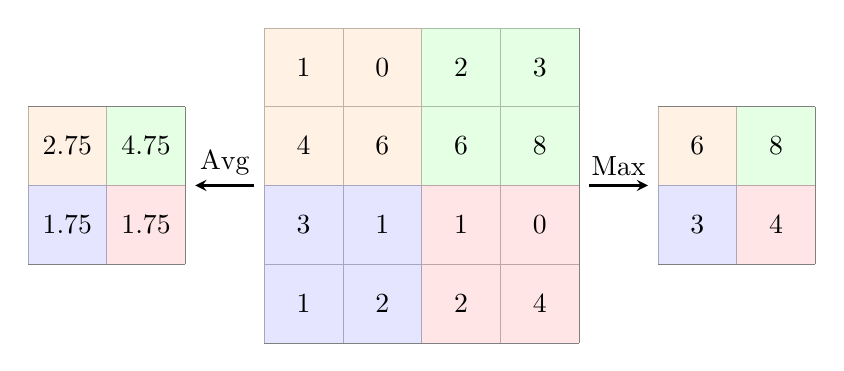
\begin{tikzpicture}
            \tikzstyle{arrow}=[thick,->,>=stealth]
            % anchor nodes
            \node (a) at (+4,2) {};
            \node (b) at (+5,2) {};
            \node (c) at (+0,2) {};
            \node (d) at (-1,2) {};
            % average pool
            \draw [arrow] (c) -- node[anchor=south]{Avg} (d);
            \draw[step=1cm,gray,very thin,xshift=-4cm] (1,1) grid (3,3);
            \fill[blue!20  ,semitransparent,xshift=-4cm] (1,1) rectangle (2,2);
            \node[xshift=-4cm] at (1.5,1.5){1.75};
            \fill[red!20   ,semitransparent,xshift=-4cm] (2,1) rectangle (3,2);
            \node[xshift=-4cm] at (2.5,1.5){1.75};
            \fill[orange!20,semitransparent,xshift=-4cm] (1,2) rectangle (2,3);
            \node[xshift=-4cm] at (1.5,2.5){2.75};
            \fill[green!20 ,semitransparent,xshift=-4cm] (2,2) rectangle (3,3);
            \node[xshift=-4cm] at (2.5,2.5){4.75};
            % original feature map
            \draw[step=1cm,gray,very thin] (0,0) grid (4,4);
            \fill[blue!20  ,semitransparent] (0,0) rectangle (2,2);
            \fill[red!20   ,semitransparent] (2,0) rectangle (4,2);
            \fill[orange!20,semitransparent] (0,2) rectangle (2,4);
            \fill[green!20 ,semitransparent] (2,2) rectangle (4,4);
            % row 1
            \node at (0.5,0.5){1};
            \node at (1.5,0.5){2};
            \node at (0.5,1.5){3};
            \node at (1.5,1.5){1};
            % row 2
            \node at (2.5,0.5){2};
            \node at (3.5,0.5){4};
            \node at (2.5,1.5){1};
            \node at (3.5,1.5){0};
            % row 3
            \node at (0.5,2.5){4};
            \node at (1.5,2.5){6};
            \node at (0.5,3.5){1};
            \node at (1.5,3.5){0};
            % row 4
            \node at (2.5,2.5){6};
            \node at (3.5,2.5){8};
            \node at (2.5,3.5){2};
            \node at (3.5,3.5){3};
            % max pool
            \draw [arrow] (a) -- node[anchor=south]{Max} (b);
            \draw[step=1cm,gray,very thin,xshift=4cm] (1,1) grid (3,3);
            \fill[blue!20  ,semitransparent,xshift=4cm] (1,1) rectangle (2,2);
            \node[xshift=4cm] at (1.5,1.5){3};
            \fill[red!20   ,semitransparent,xshift=4cm] (2,1) rectangle (3,2);
            \node[xshift=4cm] at (2.5,1.5){4};
            \fill[orange!20,semitransparent,xshift=4cm] (1,2) rectangle (2,3);
            \node[xshift=4cm] at (1.5,2.5){6};
            \fill[green!20 ,semitransparent,xshift=4cm] (2,2) rectangle (3,3);
            \node[xshift=4cm] at (2.5,2.5){8};
        \end{tikzpicture}
    \end{customcenter}
    Showing two possible pooling activation function.
\end{minipage}
%%%%%%%%%%%%%%%%%%%%%%%%%%%%%%%%%%%%
\begin{customcenter}[5pt]
    \begin{minipage}[h]{0.285\textwidth}
        \textbf{Backbone} of Mask RCNN is the feature extractor (objects instances, classes, and spatial properties). Commonly it is composed of various \textbf{Residual Network} (ResNet).
        \begin{customcenter}[5pt]
            \begin{tikzpicture}
                \tikzstyle{convnode} = [minimum width=4cm,fill=ProcessBlue!40,rounded corners,text=black]
                \tikzstyle{whitenode} = [minimum width=4cm,draw=black,text=black]
                \fill[blue!40!white,rounded corners] (-3,-0.1) rectangle (3,-3.9);
                \node[xshift=16pt,yshift=-4pt] at (-3,-0.15) {\small ResNet};
                \node [whitenode] (input) at (0,0.25) {Raw Image};
                \node [convnode] (bbn1) at (0,-0.75) {\small 7x7 convolution, 64};
                \node [convnode] (bbn2) at (0,-1.5) {\small 1x1 convolution, d};
                \node [convnode] (bbn3) at (0,-2.25) {\small 3x3 convolution, d};
                \node [convnode] (bbn4) at (0,-3.0) {\small 1x1 convolution, d'};
                \node [whitenode] (output) at (0,-4.275) {Feature Map};
                \draw (0,-3.65) node[cross=4pt,rotate=45,very thick,gray] {};
                \node [draw,circle,gray,very thick,radius=5pt] (c1) at (0,-3.65) {};
                \node [anchor=west,xshift=3pt] at (0,-3.65) {\scriptsize ReLU};

                \draw[->,very thick,] (input) -- (bbn1);
                \draw[->,very thick] (bbn1) -- node[anchor=west]{\scriptsize Channel d'} (bbn2);
                \draw[->,very thick] (bbn2) -- node[anchor=west]{\scriptsize ReLU} (bbn3);
                \draw[->,very thick] (bbn3) -- node[anchor=west]{\scriptsize ReLU} (bbn4);
                \draw[->,very thick] (bbn4) -- (c1);
                \draw[->,very thick] (c1) -- (output);

            \end{tikzpicture}
        \end{customcenter}
    \end{minipage}
    \hspace{10pt}
    \begin{minipage}[h]{0.65\textwidth}
        \begin{customcenter}[0pt]
            \begin{tabular}{|l|l|l|l|}
                \hline
                \textbf{Function} & \textbf{Definition} & \textbf{Advantages} & \textbf{Disadvantages} \\
                \hline
                Identity & $x$ & Easy to solve & Less power  to learn \\
                \hline
                Binary Step & $\begin{cases}1\quad\text{if } x\;\geq\;0 \\ 0\quad\text{if } x\;<\;0\end{cases}$ & Simple binary classifier & Discontinuous? \\
                \hline
                \multirow{3}{*}{Sigmoid} & \multirow{3}{*}{$\frac{1}{1 + e^{-x}}$} & Smooth & Values in $\bracketA{0,1}$\\
                & & Continuous & Vanishing gradient \\
                & & Non-linear & Non-symmetric and $+$ \\
                \hline\xrowht[()]{15pt}
                \hspace{-3pt}Tanh & $\frac{2}{1 + e^{-2x}} - 1$ & Same as Sigmoid & Symmetric over origin \\[0pt]
                \hline
                \multirow{3}{*}{ReLU} & \multirow{3}{*}{$\text{max}\parenthesisA{0, x}$} & Simpler computation & Exploding gradient \\
                & & Sparsity & Dying neurons \\
                & & Linearity & \\
                \hline
                Leaky ReLU & $\begin{cases}ax\quad x\;<\;0,\; a\in\mathrm{R} \\ \textcolor{white}{a}x\quad x\;\geq\;0\end{cases}$ & No dying neurons & Exploding gradient? \\
                \hline
                \multirow{2}{*}{Softmax} & \multirow{2}{*}{$\frac{e^x_j}{\sum_{k=1}^{K}e^x_j}\quad j\in\bracketA{1,K}$} & Classifier $>$ 2 classes & \multirow{2}{*}{Complex to compute?}\\
                & & Use of probabilities & \\
                \hline
            \end{tabular}
        \end{customcenter}
    \end{minipage}
\end{customcenter}